\documentclass{beamer}

\title{Cofun with Cofree Comonads}
\author{Dave Laing}
\date{YOW! Lambda Jam 2015}

\usepackage[normalem]{ulem}
\usepackage{color}
\usepackage{minted}

\setbeamertemplate{navigation symbols}{}

\AtBeginSection[]%
{%
\begin{frame}[plain]%
  \begin{center}%
    \usebeamerfont{section title}\usebeamercolor[fg]{section title}\insertsection%
  \end{center}%
\end{frame}%
}

\begin{document}

\begin{frame}
\maketitle
\end{frame}

\section{Introduction}

% The goal is not deep understanding
\begin{frame}[c]
  \centering
  A cofree functor is right adjoint to a forgetful functor.
\end{frame}

\begin{frame}[c]
  \centering
  \sout{A cofree functor is right adjoint to a forgetful functor.}
\end{frame}

% The goal is to convey intuition
\begin{frame}[c]
  \centering
  ``Cofree comonads are something I could use if I wanted to''
\end{frame}

% The goal is to seed inspiration
\begin{frame}[c]
  \centering
  ``I want to use cofree comonads for things''
\end{frame}

\begin{frame}[c]
  \centering
  Fold and unfold for lists are a good starting point
\end{frame}

\begin{frame}[c]
  \centering
  Monadic values are produced in a context
\end{frame}

\begin{frame}[c]
  \centering
  Comonadic values are consumed from a context
\end{frame}

\begin{frame}[c]
  \centering
  Combining the two can have good results
\end{frame}

% talk about the structure here

\section{Comonads}

\begin{frame}[fragile]
  \begin{overprint}
    \onslide<1>
    \begin{minted}{haskell}
class Monad m where




class Comonad w where



    \end{minted}
    \onslide<2>
    \begin{minted}{haskell}
class Monad m where
  return    :: a -> m a



class Comonad w where



    \end{minted}
    \onslide<3>
    \begin{minted}{haskell}
class Monad m where
  return    :: a -> m a



class Comonad w where
  extract   :: w a -> a


    \end{minted}
    \onslide<4>
    \begin{minted}{haskell}
class Monad m where
  return    :: a -> m a
  (>>=)     :: m a -> (a -> m b) -> m b


class Comonad w where
  extract   :: w a -> a


    \end{minted}
    \onslide<5>
    \begin{minted}{haskell}
class Monad m where
  return    :: a -> m a
  (>>=)     :: m a -> (a -> m b) -> m b


class Comonad w where
  extract   :: w a -> a
  extend    :: w a -> (w a -> b) -> w b

    \end{minted}
    \onslide<6>
    \begin{minted}{haskell}
class Monad m where
  return    :: a -> m a
  (>>=)     :: m a -> (a -> m b) -> m b
  join      :: m (m a) -> m a

class Comonad w where
  extract   :: w a -> a
  extend    :: w a -> (w a -> b) -> w b

    \end{minted}
    \onslide<7>
    \begin{minted}{haskell}
class Monad m where
  return    :: a -> m a
  (>>=)     :: m a -> (a -> m b) -> m b
  join      :: m (m a) -> m a

class Comonad w where
  extract   :: w a -> a
  extend    :: w a -> (w a -> b) -> w b
  duplicate :: w a -> w (w a)
    \end{minted}
    \end{overprint}
\end{frame}

% Uses and instances and uses
\begin{frame}[fragile]
  \begin{minted}{haskell}
data Zipper a = Zipper [a] a [a]
  \end{minted}
\end{frame}

\begin{frame}[fragile]
  \begin{overprint}
  \onslide<1>
  \begin{minted}{haskell}
z :: Zipper Int
z = Zipper [2, 1] 3 [4]

z
-- | 1 | 2 > 3 < 4 |






  \end{minted}
  \onslide<2>
  \begin{minted}{haskell}
z :: Zipper Int
z = Zipper [2, 1] 3 [4]

z
-- | 1 | 2 > 3 < 4 |

extract z
-- 3



  \end{minted}
  \onslide<3>
  \begin{minted}{haskell}
z :: Zipper Int
z = Zipper [2, 1] 3 [4]

z
-- | 1 | 2 > 3 < 4 |

extract z
-- 3

duplicate z
-- | >1<2|3|4| |1>2<3|4| > |1|2>3<4| < | |1|2|3>4< |
  \end{minted}
  \end{overprint}
\end{frame}

\begin{frame}[fragile]
\begin{overprint}
  \onslide<2>
\begin{minted}{haskell}
latch :: Ord a => Zipper a -> a
latch (Zipper l f _) =
  maximumDef f l
\end{minted}
\onslide<3>
\begin{minted}{haskell}
peak :: Ord a => Zipper a -> Bool
peak (Zipper l f r) =
  headDef f l < f && f > headDef f r
\end{minted}
\onslide<4>
\begin{minted}{haskell}
wma ::  Int -> Zipper Double -> Double
wma n (Zipper l f r) =
  average $ take n l ++ f : take n r
\end{minted}
\end{overprint}

\bigskip

\begin{overprint}
  \onslide<1>
    \begin{center}
    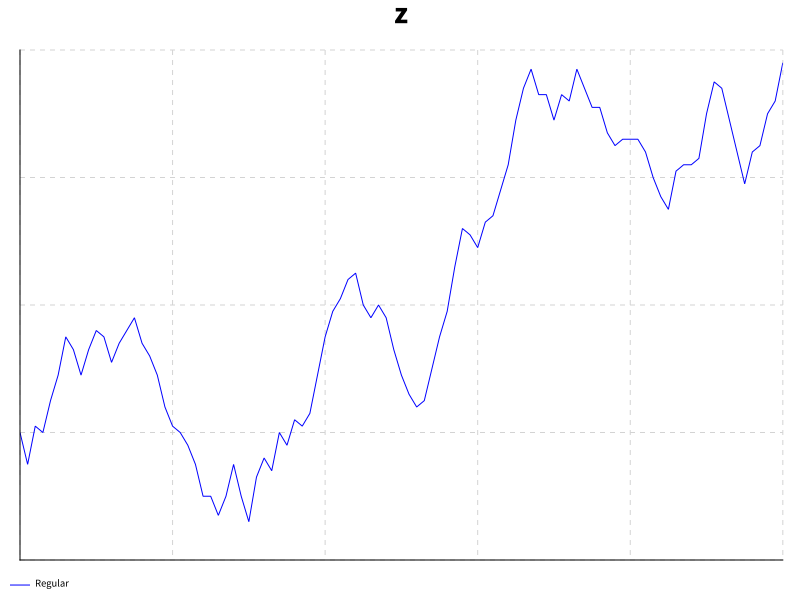
\includegraphics[width=0.75\textwidth]{graph1.png}
    \end{center}
  \onslide<2>
    \begin{center}
    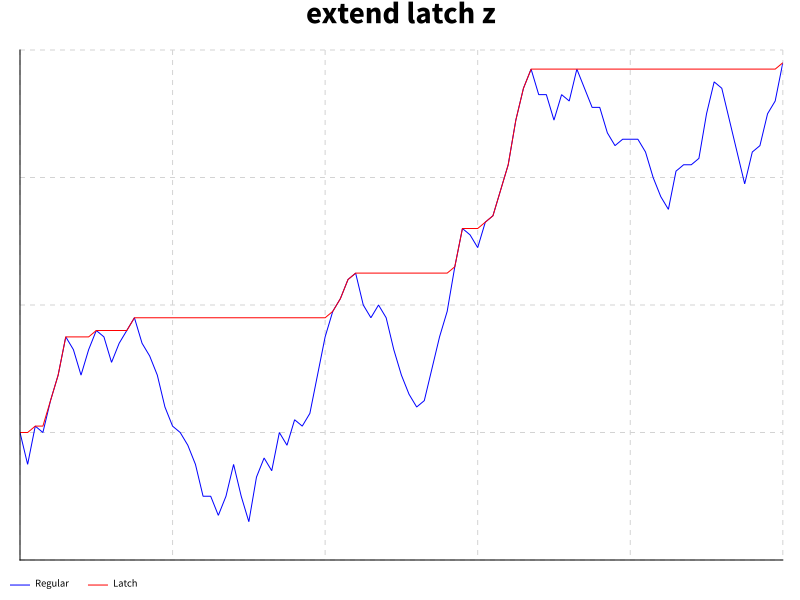
\includegraphics[width=0.75\textwidth]{graph2.png}
    \end{center}
  \onslide<3>
    \begin{center}
    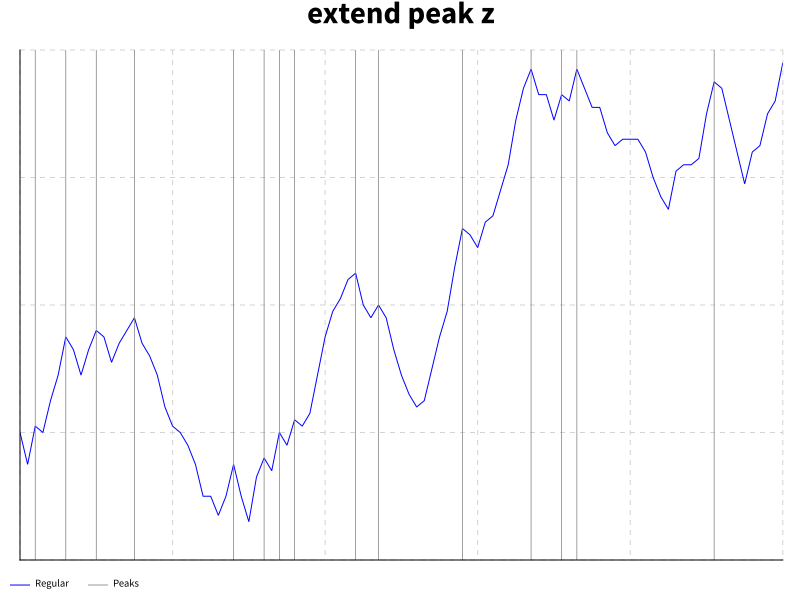
\includegraphics[width=0.75\textwidth]{graph3.png}
    \end{center}
  \onslide<4>
    \begin{center}
    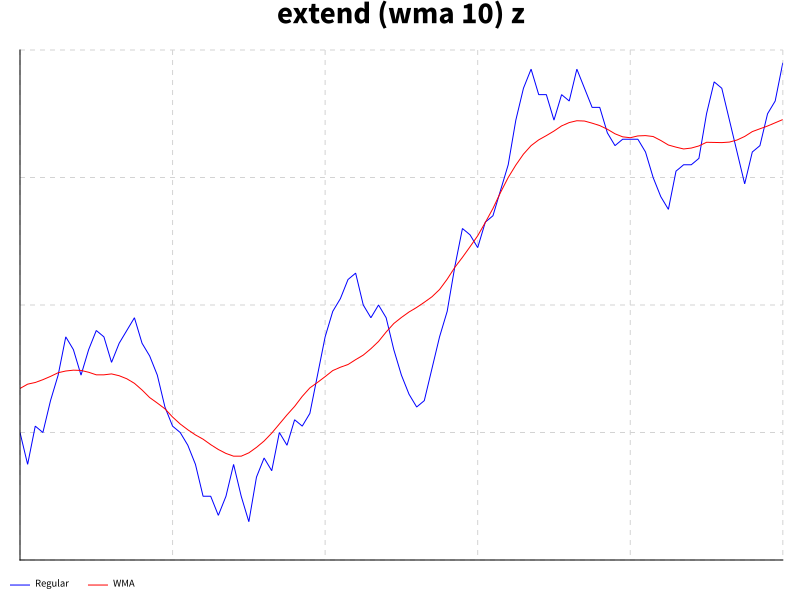
\includegraphics[width=0.75\textwidth]{graph4.png}
    \end{center}
  \onslide<5>
    \begin{center}
    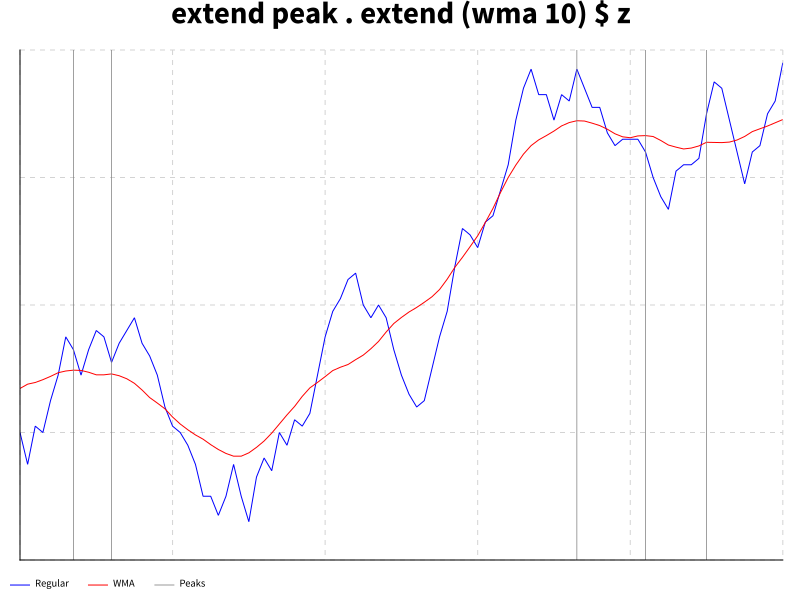
\includegraphics[width=0.75\textwidth]{graph5.png}
    \end{center}
\end{overprint}
\end{frame}

\section{Free}

\begin{frame}[fragile]
  \begin{minted}{haskell}
data Free f a =
    Pure a
  | Free (f (Free f a))

instance Functor f => Monad (Free f) where
  ...
  \end{minted}
\end{frame}

\begin{frame}[fragile]
  \begin{overprint}
    \onslide<1>
    \begin{minted}{haskell}
data AdderF k =



    \end{minted}
    \onslide<2>
    \begin{minted}{haskell}
data AdderF k =
    Add Int (Bool -> k)


    \end{minted}
    \onslide<3>
    \begin{minted}{haskell}
data AdderF k =
    Add Int (Bool -> k)
  | Clear k

    \end{minted}
    \onslide<4>
    \begin{minted}{haskell}
data AdderF k =
    Add Int (Bool -> k)
  | Clear k
  | Total (Int -> k)
    \end{minted}
  \end{overprint}
\end{frame}

\begin{frame}[fragile]
  \begin{overprint}
    \onslide<1>
    \begin{minted}{haskell}
data AdderF k = ...




instance Functor AdderF where



    \end{minted}
    \onslide<2>
    \begin{minted}{haskell}
data AdderF k =
    Add Int (Bool -> k)
    ...


instance Functor AdderF where
  fmap f (Add x k) = Add x (f . k)


    \end{minted}
    \onslide<3>
    \begin{minted}{haskell}
data AdderF k =
    Add Int (Bool -> k)
  | Clear k
  ...

instance Functor AdderF where
  fmap f (Add x k) = Add x (f . k)
  fmap f (Clear k) = Clear (f k)

    \end{minted}
    \onslide<4>
    \begin{minted}{haskell}
data AdderF k =
    Add Int (Bool -> k)
  | Clear k
  | Total (Int -> k)

instance Functor AdderF where
  fmap f (Add x k) = Add x (f . k)
  fmap f (Clear k) = Clear (f k)
  fmap f (Total k) = Total (f . k)
    \end{minted}
  \end{overprint}
\end{frame}

\begin{frame}[fragile]
  \begin{minted}{haskell}
data Free f a =
    Pure a
  | Free (f (Free f a))

instance Functor f => Monad (Free f) where
  ...
  \end{minted}
\end{frame}

\begin{frame}[fragile]
  \begin{overprint}
    \onslide<1>
  \begin{minted}{haskell}
type Adder a = Free AdderF a




  \end{minted}
    \onslide<2>
  \begin{minted}{haskell}
type Adder a =
    Pure a
  | Free (AdderF (Adder a))


  \end{minted}
    \onslide<3>
  \begin{minted}{haskell}
type Adder a =
    Pure a
  | Free (Add Int (Bool -> Adder a))
  | Free (Clear (Adder a))
  | Free (Total (Int -> Adder a))
  \end{minted}
  \end{overprint}
\end{frame}

\section{Using Free}

\begin{frame}[fragile]
  \begin{minted}{haskell}
add :: Int -> Adder Bool
add x = liftF $ Add x id

clear :: Adder ()
clear = liftF $ Clear ()

total :: Adder Int
total = liftF $ Total id
  \end{minted}
\end{frame}

\begin{frame}[fragile]
  \begin{overprint}
    \onslide<1>
  \begin{minted}{haskell}
findLimit :: Adder Int
findLimit = do











  \end{minted}
    \onslide<2>
  \begin{minted}{haskell}
findLimit :: Adder Int
findLimit = do
  -- capture the old count
  t <- total
  -- clear the count
  clear







  \end{minted}
    \onslide<3>
  \begin{minted}{haskell}
findLimit :: Adder Int
findLimit = do
  -- capture the old count
  t <- total
  -- clear the count
  clear
  -- seek out the limit
  r <- execStateT findLimit' 0





  \end{minted}
    \onslide<4>
  \begin{minted}{haskell}
findLimit :: Adder Int
findLimit = do
  -- capture the old count
  t <- total
  -- clear the count
  clear
  -- seek out the limit
  r <- execStateT findLimit' 0
  -- restore the old count
  clear
  _ <- add t


  \end{minted}
    \onslide<5>
  \begin{minted}{haskell}
findLimit :: Adder Int
findLimit = do
  -- capture the old count
  t <- total
  -- clear the count
  clear
  -- seek out the limit
  r <- execStateT findLimit' 0
  -- restore the old count
  clear
  _ <- add t
  -- return the result
  return r
  \end{minted}
  \end{overprint}
\end{frame}

\begin{frame}[fragile]
  \begin{overprint}
    \onslide<1>
  \begin{minted}{haskell}
findLimit' :: StateT Int Adder ()
findLimit' = do








  \end{minted}
    \onslide<2>
  \begin{minted}{haskell}
findLimit' :: StateT Int Adder ()
findLimit' = do
  -- add 1 to the total
  r <- lift $ add 1






  \end{minted}
    \onslide<3>
  \begin{minted}{haskell}
findLimit' :: StateT Int Adder ()
findLimit' = do
  -- add 1 to the total
  r <- lift $ add 1
  -- check for overflow
  when r $ do




  \end{minted}
    \onslide<4>
  \begin{minted}{haskell}
findLimit' :: StateT Int Adder ()
findLimit' = do
  -- add 1 to the total
  r <- lift $ add 1
  -- check for overflow
  when r $ do
    -- if no overflow, add to our state counter ...
    modify (+ 1)


  \end{minted}
    \onslide<5>
  \begin{minted}{haskell}
findLimit' :: StateT Int Adder ()
findLimit' = do
  -- add 1 to the total
  r <- lift $ add 1
  -- check for overflow
  when r $ do
    -- if no overflow, add to our state counter ...
    modify (+ 1)
    -- and continue
    findLimit'
  \end{minted}
  \end{overprint}
\end{frame}

\begin{frame}[c]
  \centering
  Separation of the client code from the interpreter code
\end{frame}

\begin{frame}[c]
  \centering
  Reuse code written in terms of the client code
\end{frame}

\begin{frame}[c]
  \centering
  Write different interpreters for different needs
\end{frame}

\section{Cofree}

\begin{frame}[fragile]
  \begin{minted}{haskell}
data Cofree f a = a :< f (Cofree f a)

instance Functor f => Comonad (Cofree f)
  ...
  \end{minted}
\end{frame}

\begin{frame}[fragile]
  \begin{overprint}
    \onslide<1>
  \begin{minted}{haskell}
data CoAdderF k = CoAdderF {




  \end{minted}
    \onslide<2>
  \begin{minted}{haskell}
data CoAdderF k = CoAdderF {
    addH   :: Int -> (Bool, k)



  \end{minted}
    \onslide<3>
  \begin{minted}{haskell}
data CoAdderF k = CoAdderF {
    addH   :: Int -> (Bool, k)
  , clearH :: k


  \end{minted}
    \onslide<4>
  \begin{minted}{haskell}
data CoAdderF k = CoAdderF {
    addH   :: Int -> (Bool, k)
  , clearH :: k
  , totalH :: (Int, k)
  }
  \end{minted}
  \end{overprint}
\end{frame}

\begin{frame}[fragile]
  \begin{overprint}
    \onslide<1>
  \begin{minted}{haskell}
data CoAdderF k = CoAdderF {
    ...
  }



instance Functor CoAdderF where
  fmap f (CoAdderF a c t) = CoAdderF



  \end{minted}
    \onslide<2>
  \begin{minted}{haskell}
data CoAdderF k = CoAdderF {
    addH   :: Int -> (Bool, k)
    ...
  }


instance Functor CoAdderF where
  fmap f (CoAdderF a c t) = CoAdderF
    (fmap (fmap f) a)


  \end{minted}
    \onslide<3>
  \begin{minted}{haskell}
data CoAdderF k = CoAdderF {
    addH   :: Int -> (Bool, k)
  , clearH :: k
    ...
  }

instance Functor CoAdderF where
  fmap f (CoAdderF a c t) = CoAdderF
    (fmap (fmap f) a)
    (f c)

  \end{minted}
    \onslide<4>
  \begin{minted}{haskell}
data CoAdderF k = CoAdderF {
    addH   :: Int -> (Bool, k)
  , clearH :: k
  , totalH :: (Int, k)
  }

instance Functor CoAdderF where
  fmap f (CoAdderF a c t) = CoAdderF
    (fmap (fmap f) a)
    (f c)
    (fmap f t)
  \end{minted}
  \end{overprint}
\end{frame}

\begin{frame}[fragile]
  \begin{minted}{haskell}
data Cofree f a = a :< f (Cofree f a)

instance Functor f => Comonad (Cofree f)
  ...
  \end{minted}
\end{frame}

\begin{frame}[fragile]
  \begin{overprint}
    \onslide<1>
  \begin{minted}{haskell}
type CoAdder a = Cofree CoAdderF a




  \end{minted}
    \onslide<2>
  \begin{minted}{haskell}
type CoAdder a = a :< CoAdderF (CoAdder a)




  \end{minted}
    \onslide<3>
  \begin{minted}{haskell}
type CoAdder a = a :< CoAdderF {
    Int -> (Bool, CoAdder a)
  , CoAdder a
  , (Int, CoAdder a)
  }
  \end{minted}
  \end{overprint}
\end{frame}

\section{Using Cofree}

\begin{frame}[fragile]
  \begin{overprint}
    \onslide<1>
  \begin{minted}{haskell}
type Limit = Int
type Count = Int



mkCoAdder :: Limit -> Count -> CoAdder (Limit, Count)
mkCoAdder limit count = _





  \end{minted}
    \onslide<2>
  \begin{minted}{haskell}
type Limit = Int
type Count = Int

coiter :: Functor f => (a -> f a) -> a -> Cofree f a

mkCoAdder :: Limit -> Count -> CoAdder (Limit, Count)
mkCoAdder limit count = _





  \end{minted}
    \onslide<3>
  \begin{minted}{haskell}
type Limit = Int
type Count = Int

coiter :: Functor f => (a -> f a) -> a -> Cofree f a

mkCoAdder :: Limit -> Count -> CoAdder (Limit, Count)
mkCoAdder limit count =
          coiter next start




  \end{minted}
    \onslide<4>
  \begin{minted}{haskell}
type Limit = Int
type Count = Int

coiter :: Functor f => (a -> f a) -> a -> Cofree f a

mkCoAdder :: Limit -> Count -> CoAdder (Limit, Count)
mkCoAdder limit count =
          coiter next start

  where
    next w = CoAdderF _ _ _
    start (limit, count)
  \end{minted}
    \onslide<5>
  \begin{minted}{haskell}
type Limit = Int
type Count = Int

coiter :: Functor f => (a -> f a) -> a -> Cofree f a

mkCoAdder :: Limit -> Count -> CoAdder (Limit, Count)
mkCoAdder limit count =
    start
      :< (coiter next <$> next start)
  where
    next w = CoAdderF _ _ _
    start (limit, count)
  \end{minted}
    \onslide<6>
  \begin{minted}{haskell}
type Limit = Int
type Count = Int

coiter :: Functor f => (a -> f a) -> a -> Cofree f a

mkCoAdder :: Limit -> Count -> CoAdder (Limit, Count)
mkCoAdder limit count =
    start :< next start
      :< (coiter next <$> next (next start))
  where
    next w = CoAdderF _ _ _
    start (limit, count)
  \end{minted}
    \onslide<7>
  \begin{minted}{haskell}
type Limit = Int
type Count = Int

coiter :: Functor f => (a -> f a) -> a -> Cofree f a

mkCoAdder :: Limit -> Count -> CoAdder (Limit, Count)
mkCoAdder limit count =
          coiter next start

  where
    next w = CoAdderF (coAdd w) (coClear w) (coTotal w)
    start (limit, count)
  \end{minted}
  \end{overprint}
\end{frame}

\begin{frame}[fragile]
  \begin{overprint}
    \onslide<1>
    \begin{minted}{haskell}
next w = CoAdderF (coAdd w) (coClear w) (coTotal w)

coClear :: (Limit, Count) -> (Limit, Count)


coTotal :: (Limit, Count) -> (Int, (Limit, Count))


coAdd :: (Limit, Count) -> Int -> (Bool, (Limit, Count))





  \end{minted}
    \onslide<2>
    \begin{minted}{haskell}
next w = CoAdderF (coAdd w) (coClear w) (coTotal w)

coClear :: (Limit, Count) -> (Limit, Count)
coClear (limit, count) = (limit, 0)

coTotal :: (Limit, Count) -> (Int, (Limit, Count))


coAdd :: (Limit, Count) -> Int -> (Bool, (Limit, Count))





  \end{minted}
    \onslide<3>
    \begin{minted}{haskell}
next w = CoAdderF (coAdd w) (coClear w) (coTotal w)

coClear :: (Limit, Count) -> (Limit, Count)
coClear (limit, count) = (limit, 0)

coTotal :: (Limit, Count) -> (Int, (Limit, Count))
coTotal (limit, count) = (count, (limit, count))

coAdd :: (Limit, Count) -> Int -> (Bool, (Limit, Count))





  \end{minted}
    \onslide<4>
    \begin{minted}{haskell}
next w = CoAdderF (coAdd w) (coClear w) (coTotal w)

coClear :: (Limit, Count) -> (Limit, Count)
coClear (limit, count) = (limit, 0)

coTotal :: (Limit, Count) -> (Int, (Limit, Count))
coTotal (limit, count) = (count, (limit, count))

coAdd :: (Limit, Count) -> Int -> (Bool, (Limit, Count))
coAdd (limit, count) x = (_   , (limit, _   ))




    \end{minted}
    \onslide<5>
    \begin{minted}{haskell}
next w = CoAdderF (coAdd w) (coClear w) (coTotal w)

coClear :: (Limit, Count) -> (Limit, Count)
coClear (limit, count) = (limit, 0)

coTotal :: (Limit, Count) -> (Int, (Limit, Count))
coTotal (limit, count) = (count, (limit, count))

coAdd :: (Limit, Count) -> Int -> (Bool, (Limit, Count))
coAdd (limit, count) x = (_   , (limit, _   ))
  where
    count' = count + x
    test   = count' <= limit

  \end{minted}
    \onslide<6>
    \begin{minted}{haskell}
next w = CoAdderF (coAdd w) (coClear w) (coTotal w)

coClear :: (Limit, Count) -> (Limit, Count)
coClear (limit, count) = (limit, 0)

coTotal :: (Limit, Count) -> (Int, (Limit, Count))
coTotal (limit, count) = (count, (limit, count))

coAdd :: (Limit, Count) -> Int -> (Bool, (Limit, Count))
coAdd (limit, count) x = (test, (limit, _   ))
  where
    count' = count + x
    test   = count' <= limit

  \end{minted}
    \onslide<7>
    \begin{minted}{haskell}
next w = CoAdderF (coAdd w) (coClear w) (coTotal w)

coClear :: (Limit, Count) -> (Limit, Count)
coClear (limit, count) = (limit, 0)

coTotal :: (Limit, Count) -> (Int, (Limit, Count))
coTotal (limit, count) = (count, (limit, count))

coAdd :: (Limit, Count) -> Int -> (Bool, (Limit, Count))
coAdd (limit, count) x = (test, (limit, _   ))
  where
    count' = count + x
    test   = count' <= limit
    next   = if test then count' else count
  \end{minted}
    \onslide<8>
    \begin{minted}{haskell}
next w = CoAdderF (coAdd w) (coClear w) (coTotal w)

coClear :: (Limit, Count) -> (Limit, Count)
coClear (limit, count) = (limit, 0)

coTotal :: (Limit, Count) -> (Int, (Limit, Count))
coTotal (limit, count) = (count, (limit, count))

coAdd :: (Limit, Count) -> Int -> (Bool, (Limit, Count))
coAdd (limit, count) x = (test, (limit, next))
  where
    count' = count + x
    test   = count' <= limit
    next   = if test then count' else count
  \end{minted}
  \end{overprint}
\end{frame}

\begin{frame}[c]
  \centering
  Separation of the interpreter code from the client code
\end{frame}

\begin{frame}[c]
  \centering
  Reuse code written in terms of the interpreter code
\end{frame}

\begin{frame}[c]
  \centering
  Write different clients for different needs
\end{frame}

\section{Comonad transformers}

\subsection{Relation to monad transformers}

\begin{frame}[fragile]
  \begin{minted}{haskell}
class MonadTrans t where
  lift :: Monad m => m a -> t m a

class ComonadTrans t where
  lower :: Comonad w => t w a -> w a
  \end{minted}
\end{frame}

\subsection{Instances}

\subsection{CoAdder}

\begin{frame}[fragile]
  \begin{overprint}
    \onslide<1>
  \begin{minted}{haskell}
type Limit = Int
type Count = Int

type CoAdder = Cofree CoAdderF


mkCoAdder :: Limit -> Count -> CoAdder ()
mkCoAdder limit count =
    () <$ coiter  next start
  where
    next w = CoAdderF (coAdd w) (coClear w) (coTotal w)
    start (limit, count)


  \end{minted}
    \onslide<2>
  \begin{minted}{haskell}
type Limit = Int
type Count = Int

type CoAdder = CofreeT CoAdderF Base
type Base = StoreT Count (EnvT Limit Identity)

mkCoAdder :: Limit -> Count -> CoAdder ()
mkCoAdder limit count =
    () <$ coiter  next start
  where
    next w = CoAdderF (coAdd w) (coClear w) (coTotal w)
    start (limit, count)


  \end{minted}
    \onslide<3>
  \begin{minted}{haskell}
type Limit = Int
type Count = Int

type CoAdder = CofreeT CoAdderF Base
type Base = StoreT Count (EnvT Limit Identity)

mkCoAdder :: Limit -> Count -> CoAdder ()
mkCoAdder limit count =
          coiterT next start
  where
    next w = CoAdderF (coAdd w) (coClear w) (coTotal w)
    start (limit, count)


  \end{minted}
  \onslide<4>
  \begin{minted}{haskell}
type Limit = Int
type Count = Int

type CoAdder = CofreeT CoAdderF Base
type Base = StoreT Count (EnvT Limit Identity)

mkCoAdder :: Limit -> Count -> CoAdder ()
mkCoAdder limit count =
          coiterT next start
  where
    next w = CoAdderF (coAdd w) (coClear w) (coTotal w)
    start = flip StoreT count .
            EnvT limit .
            Identity $
            const ()
  \end{minted}
  \end{overprint}
\end{frame}

% coClear and coTotal
% compare seek / pos to set / get
% before and after

\begin{frame}[fragile]
  \begin{minted}{haskell}
coClear :: (Limit, Count) -> (Limit, Count)
coClear (limit, count) = (limit, 0)

coTotal :: (Limit, Count) -> (Int, (Limit, Count))
coTotal (limit, count) = (count, (limit, count))
  \end{minted}
\end{frame}

\begin{frame}[fragile]
  \begin{overprint}
    \onslide<1>
  \begin{minted}{haskell}
    get  :: StateT s m s
    set  :: s -> StateT s m ()
  \end{minted}
    \onslide<2>
  \begin{minted}{haskell}
    pos  :: StoreT s w a -> s
    set  :: s -> StateT s m ()
  \end{minted}
    \onslide<3>
  \begin{minted}{haskell}
    pos  :: StoreT s w a -> s
    seek :: s -> StoreT s w a  -> StoreT s w a
  \end{minted}
  \end{overprint}
\end{frame}

\begin{frame}[fragile]
  \begin{overprint}
    \onslide<1>
  \begin{minted}{haskell}
type Limit, Count = Int

coClear :: (Limit, Count) -> (Limit, Count)
coClear (limit, count) = (limit, 0)

coTotal :: (Limit, Count) -> (Int, (Limit, Count))
coTotal (limit, count) = (count, (limit, count))
  \end{minted}
    \onslide<2>
  \begin{minted}{haskell}
type Base = StoreT Count (EnvT Limit Identity)

coClear :: (Limit, Count) -> (Limit, Count)
coClear (limit, count) = (limit, 0)

coTotal :: (Limit, Count) -> (Int, (Limit, Count))
coTotal (limit, count) = (count, (limit, count))
  \end{minted}
    \onslide<3>
  \begin{minted}{haskell}
type Base = StoreT Count (EnvT Limit Identity)

coClear :: Base a         -> Base a
coClear (limit, count) = (limit, 0)

coTotal :: (Limit, Count) -> (Int, (Limit, Count))
coTotal (limit, count) = (count, (limit, count))
  \end{minted}
    \onslide<4>
  \begin{minted}{haskell}
type Base = StoreT Count (EnvT Limit Identity)

coClear :: Base a         -> Base a
coClear w              = seek 0 w

coTotal :: (Limit, Count) -> (Int, (Limit, Count))
coTotal (limit, count) = (count, (limit, count))
  \end{minted}
    \onslide<5>
  \begin{minted}{haskell}
type Base = StoreT Count (EnvT Limit Identity)

coClear :: Base a         -> Base a
coClear w              = seek 0 w

coTotal :: Base a         -> (Int, Base a)
coTotal (limit, count) = (count, (limit, count))
  \end{minted}
    \onslide<6>
  \begin{minted}{haskell}
type Base = StoreT Count (EnvT Limit Identity)

coClear :: Base a         -> Base a
coClear w              = seek 0 w

coTotal :: Base a         -> (Int, Base a)
coTotal w              = (pos w, w)
  \end{minted}

  \end{overprint}
\end{frame}

% coAdd
% explain ask
% before and after

\begin{frame}[fragile]
  \begin{minted}{haskell}
coAdd :: (Limit, Count) -> Int -> (Bool, (Limit, Count))
coAdd (limit, count) x = (test, (limit, next))
  where
    count' = count + x
    test   = count' <= limit
    next   = if test then count' else count
  \end{minted}
\end{frame}

\begin{frame}[fragile]
  \begin{overprint}
    \onslide<1>
  \begin{minted}{haskell}
    ask  :: ReaderT r m r
  \end{minted}
    \onslide<2>
  \begin{minted}{haskell}
    ask  :: EnvT e w a -> e
  \end{minted}
  \end{overprint}
\end{frame}

\begin{frame}[fragile]
  \begin{overprint}
    \onslide<1>
    \begin{minted}{haskell}
type Limit, Count = Int

coAdd :: (Limit, Count) -> Int -> (Bool, (Limit, Count))
coAdd (limit, count) x = (test, (limit, next))
  where


    count' = count + x
    test   = count' <= limit
    next   = if test then count' else count
    \end{minted}
    \onslide<2>
    \begin{minted}{haskell}
type Base = StoreT Count (EnvT Limit Identity)

coAdd :: (Limit, Count) -> Int -> (Bool, (Limit, Count))
coAdd (limit, count) x = (test, (limit, next))
  where


    count' = count + x
    test   = count' <= limit
    next   = if test then count' else count
    \end{minted}
    \onslide<3>
    \begin{minted}{haskell}
type Base = StoreT Count (EnvT Limit Identity)

coAdd :: Base a         -> Int -> (Bool, Base a)
coAdd (limit, count) x = (test, (limit, next))
  where


    count' = count + x
    test   = count' <= limit
    next   = if test then count' else count
    \end{minted}
    \onslide<4>
    \begin{minted}{haskell}
type Base = StoreT Count (EnvT Limit Identity)

coAdd :: Base a         -> Int -> (Bool, Base a)
coAdd w              x = (test, seek next w)
  where
    count  = _
    limit  = _
    count' = count + x
    test   = count' <= limit
    next   = if test then count' else count
  \end{minted}
    \onslide<5>
  \begin{minted}{haskell}
type Base = StoreT Count (EnvT Limit Identity)

coAdd :: Base a         -> Int -> (Bool, Base a)
coAdd w              x = (test, seek next w)
  where
    count  = pos w
    limit  = ask . lower $ w
    count' = count + x
    test   = count' <= limit
    next   = if test then count' else count
  \end{minted}
  \end{overprint}
\end{frame}


\subsection{Transformers verus MTL style}

\begin{frame}[fragile]
  \begin{overprint}
    \onslide<1>
  \begin{minted}{haskell}
type Base = StoreT Count (EnvT Limit Identity)

coClear ::
           Base a -> Base a
coClear = seek 0

coTotal ::
           Base a -> (Int, Base a)
coTotal w = (pos w, w)

coAdd ::
         Base a -> Int -> (Bool, Base a)
coAdd w x = (test, seek next w)
  where
    count  = pos w
    limit  = ask . lower $ w
    count' = count + x
    test   = count' <= limit
    next   = if test then count' else count
  \end{minted}
    \onslide<2>
  \begin{minted}{haskell}
type Base = StoreT Count (EnvT Limit Identity)

coClear :: ComonadStore Count w
        => Base a -> Base a
coClear = seek 0

coTotal :: ComonadStore Count w
        => Base a -> (Int, Base a)
coTotal w = (pos w, w)

coAdd :: (ComonadEnv Limit w, ComonadStore Count w)
      => Base a -> Int -> (Bool, Base a)
coAdd w x = (test, seek next w)
  where
    count  = pos w
    limit  = ask . lower $ w
    count' = count + x
    test   = count' <= limit
    next   = if test then count' else count
  \end{minted}
    \onslide<3>
  \begin{minted}{haskell}
type Base = StoreT Count (EnvT Limit Identity)

coClear :: ComonadStore Count w
        => w    a -> w    a
coClear = seek 0

coTotal :: ComonadStore Count w
        => w    a -> (Int, w    a)
coTotal w = (pos w, w)

coAdd :: (ComonadEnv Limit w, ComonadStore Count w)
      => w    a -> Int -> (Bool, w    a)
coAdd w x = (test, seek next w)
  where
    count  = pos w
    limit  = ask . lower $ w
    count' = count + x
    test   = count' <= limit
    next   = if test then count' else count
  \end{minted}
  \onslide<4>
    \begin{minted}{haskell}
type Base = StoreT Count (EnvT Limit Identity)

coClear :: ComonadStore Count w
        => w    a -> w    a
coClear = seek 0

coTotal :: ComonadStore Count w
        => w    a -> (Int, w    a)
coTotal w = (pos w, w)

coAdd :: (ComonadEnv Limit w, ComonadStore Count w)
      => w    a -> Int -> (Bool, w    a)
coAdd w x = (test, seek next w)
  where
    count  = pos w
    limit  = ask w
    count' = count + x
    test   = count' <= limit
    next   = if test then count' else count
  \end{minted}
  \end{overprint}
\end{frame}

\section{Pairing}

\begin{frame}[fragile]
  \begin{overprint}
    \onslide<1>
  \begin{minted}{haskell}
class (Functor f, Functor g) => Pairing f g where
    pair :: (a -> b -> r) -> f a -> g b -> r



  \end{minted}
    \onslide<2>
  \begin{minted}{haskell}
class (Functor f, Functor g) => Pairing f g where
    pair :: (a -> b -> r) -> f a -> g b -> r

instance Pairing Identity Identity where
  pair f (Identity a) (Identity b) = f a b
  \end{minted}
  \end{overprint}
\end{frame}

\begin{frame}[fragile]
  \begin{overprint}
    \onslide<1>
  \begin{minted}{haskell}
instance Pairing ((->) a) ((,) a) where
  pair p f = uncurry (p . f)



  \end{minted}
    \onslide<2>
  \begin{minted}{haskell}
instance Pairing ((->) a) ((,) a) where
  pair p f = uncurry (p . f)

instance Pairing ((,) a) ((->) a) where
  pair p f g = p (snd f) (g (fst f))
  \end{minted}
    \onslide<3>
  \begin{minted}{haskell}
instance Pairing ((->) a) ((,) a) where
  pair p f = uncurry (p . f)

instance Pairing ((,) a) ((->) a) where
  pair p f g = pair (flip p) g f
  \end{minted}
  \end{overprint}
\end{frame}

\begin{frame}[fragile]
  \begin{overprint}
    \onslide<1>
  \begin{minted}{haskell}
instance Pairing f g => Pairing (Cofree f) (Free g) where


  \end{minted}
    \onslide<2>
  \begin{minted}{haskell}
instance Pairing f g => Pairing (Cofree f) (Free g) where
  pair p (a :< _)  (Pure x)  = p a x

  \end{minted}
    \onslide<3>
  \begin{minted}{haskell}
instance Pairing f g => Pairing (Cofree f) (Free g) where
  pair p (a :< _)  (Pure x)  = p a x
  pair p (_ :< fs) (Free gs) = pair (pair p) fs gs
  \end{minted}
  \end{overprint}
\end{frame}


\begin{frame}[fragile]
  \begin{overprint}
    \onslide<1>
  \begin{minted}{haskell}
data AdderF k =          data CoAdderF k = CoAdderF {





instance Pairing CoAdderF AdderF where



  \end{minted}
    \onslide<2>
  \begin{minted}{haskell}
data AdderF k =          data CoAdderF k = CoAdderF {
    Add Int (Bool -> k)      addH   :: Int -> (Bool,k)




instance Pairing CoAdderF AdderF where



  \end{minted}
    \onslide<3>
  \begin{minted}{haskell}
data AdderF k =          data CoAdderF k = CoAdderF {
    Add Int (Bool -> k)      addH   :: Int -> (Bool,k)




instance Pairing CoAdderF AdderF where
  pair f (CoAdderF a _ _) (Add x k) = pair f (a x) k


  \end{minted}
    \onslide<4>
  \begin{minted}{haskell}
data AdderF k =          data CoAdderF k = CoAdderF {
    Add Int (Bool -> k)      addH   :: Int -> (Bool,k)
  | Clear k                , clearH :: k



instance Pairing CoAdderF AdderF where
  pair f (CoAdderF a _ _) (Add x k) = pair f (a x) k


  \end{minted}
    \onslide<5>
  \begin{minted}{haskell}
data AdderF k =          data CoAdderF k = CoAdderF {
    Add Int (Bool -> k)      addH   :: Int -> (Bool,k)
  | Clear k                , clearH :: k



instance Pairing CoAdderF AdderF where
  pair f (CoAdderF a _ _) (Add x k) = pair f (a x) k
  pair f (CoAdderF _ c _) (Clear k) = f c k

  \end{minted}
    \onslide<6>
  \begin{minted}{haskell}
data AdderF k =          data CoAdderF k = CoAdderF {
    Add Int (Bool -> k)      addH   :: Int -> (Bool,k)
  | Clear k                , clearH :: k
  | Total (Int -> k)       , totalH :: (Int,k)
                           }

instance Pairing CoAdderF AdderF where
  pair f (CoAdderF a _ _) (Add x k) = pair f (a x) k
  pair f (CoAdderF _ c _) (Clear k) = f c k

  \end{minted}
    \onslide<7>
  \begin{minted}{haskell}
data AdderF k =          data CoAdderF k = CoAdderF {
    Add Int (Bool -> k)      addH   :: Int -> (Bool,k)
  | Clear k                , clearH :: k
  | Total (Int -> k)       , totalH :: (Int,k)
                           }

instance Pairing CoAdderF AdderF where
  pair f (CoAdderF a _ _) (Add x k) = pair f (a x) k
  pair f (CoAdderF _ c _) (Clear k) = f c k
  pair f (CoAdderF _ _ t) (Total k) = pair f t k
  \end{minted}
  \end{overprint}
\end{frame}


% running cofree with free
\begin{frame}[fragile]
  \begin{minted}{haskell}
runLimit :: CoAdder a -> Int
runLimit w = pair (\_ b -> b) w findLimit

testLimit :: Int -> Bool
testLimit x = runLimit (mkCoAdder x 0) == x
  \end{minted}
\end{frame}

\begin{frame}[fragile]
  \begin{minted}{haskell}
pairEffect :: (Pairing f g, Comonad w, Monad m)
           => (a -> b -> r)
           -> CofreeT f w a
           -> FreeT g m b -> m r
pairEffect p s c = do
    mb <- runFreeT c
    case mb of
        Pure x -> return $ p (extract s) x
        Free gs -> pair (pairEffect p) (unwrap s) gs
  \end{minted}
\end{frame}

\begin{frame}[fragile]
  \begin{minted}{haskell}
consoleAdder :: MonadIO m => AdderT m ()
consoleAdder = do
    l <- liftIO getLine
    case words l of
      ["add", x] -> add (read x) >>= \b ->
        output $ "add result: " ++ show b
      ["clear"]  -> clear
      ["total"]  -> total >>= \t ->
        output $ "total result: " ++ show t
      _          -> output prompt
  where
    output = liftIO . putStrLn
    prompt = unlines
      ["Commands:", "  add [int]", "  clear", "  total"]
  \end{minted}
\end{frame}

\begin{frame}[fragile]
  \begin{minted}{haskell}
testConsole :: IO ()
testConsole = pairEffect (\_ _ -> r)
  (mkCoAdder 10 0)
  (forever consoleAdder)
  \end{minted}
\end{frame}

\section{Coproducts}

\begin{frame}[fragile]
  \begin{overprint}
    \onslide<1>
  \begin{minted}{haskell}
data AddF k = Add Int (Bool -> k)



data CoAddF k = CoAdd (Int -> (Bool, k))




  \end{minted}
    \onslide<2>
  \begin{minted}{haskell}
data AddF k = Add Int (Bool -> k)

instance Functor AddF where ...

data CoAddF k = CoAdd (Int -> (Bool, k))

instance Functor CoAddF where ...


  \end{minted}
    \onslide<3>
  \begin{minted}{haskell}
data AddF k = Add Int (Bool -> k)

instance Functor AddF where ...

data CoAddF k = CoAdd (Int -> (Bool, k))

instance Functor CoAddF where ...

instance Pairing CoAddF AddF where ...
  \end{minted}
  \end{overprint}
\end{frame}

\begin{frame}[fragile]
  \begin{overprint}
    \onslide<1>
  \begin{minted}{haskell}
type AdderF   =  AddF  :+: ClearF   :+: TotalF

type CoAdderF = CoAddF :*: CoClearF :*: CoTotalF





  \end{minted}
    \onslide<2>
  \begin{minted}{haskell}
type AdderF   =  AddF  :+: ClearF   :+: TotalF

type CoAdderF = CoAddF :*: CoClearF :*: CoTotalF

instance (Pairing f1 g1, Pairing f2, g2) =>
         Pairing (f1 :+: f2) (g1 :*: g2) where ...


  \end{minted}
    \onslide<3>
  \begin{minted}{haskell}
type AdderF   =  AddF  :+: ClearF   :+: TotalF

type CoAdderF = CoAddF :*: CoClearF :*: CoTotalF

instance (Pairing f1 g1, Pairing f2, g2) =>
         Pairing (f1 :+: f2) (g1 :*: g2) where ...

-- give us an instance of Pairing for CoAdderF and AdderF
  \end{minted}
  \end{overprint}
\end{frame}

\begin{frame}[fragile]
  \begin{minted}{haskell}
class (Functor sub, Functor sup) => sub :<: sup where
  inj :: sub a -> sup a

add :: (Functor f, AddF :<: f) => Int -> Free f Bool
add x = liftF . inj $ Add x id
  \end{minted}
\end{frame}

\begin{frame}[fragile]
  \begin{minted}{haskell}
(*:*) :: (Functor f, Functor g) =>
    (a -> f a) -> (a -> g a) -> a -> (f :*: g) a
(*:*) = liftA2 (:*:)

coAdd :: (Int, Int) -> CoAddF (Int, Int)

mkCoAdder :: Int -> Int -> CoAdder (Int, Int)
mkCoAdder limit count =
  coiter (coAdd *:* coClear *:* coTotal) (limit, count)
  \end{minted}
\end{frame}

\section{More cofun}

\begin{frame}[c]
  \centering
  Networking
\end{frame}

\begin{frame}[fragile]
  \begin{overprint}
    \onslide<1>
  \begin{minted}{haskell}
data AddReq = AddReq Int



data AddRes = AddRes Bool


  \end{minted}
    \onslide<2>
  \begin{minted}{haskell}
data AddReq = AddReq Int

instance Binary AddReq where ...

data AddRes = AddRes Bool

instance Binary AddRes where ...
  \end{minted}
  \end{overprint}
\end{frame}

\begin{frame}[fragile]
  \begin{overprint}
    \onslide<1>
  \begin{minted}{haskell}
data AddClientF m k =
  AddClientF AddReq (m (Either NetError AddRes -> k))



data CoAddClientF m k =
  CoAddClientF (AddReq -> m (Either NetError AddRes, k))



  \end{minted}
    \onslide<2>
  \begin{minted}{haskell}
data AddClientF m k =
  AddClientF AddReq (m (Either NetError AddRes -> k))

instance Functor m => Functor (AddClientF m) where ...

data CoAddClientF m k =
  CoAddClientF (AddReq -> m (Either NetError AddRes, k))

instance Functor m => Functor (CoAddClientF m) where ...


  \end{minted}
    \onslide<3>
  \begin{minted}{haskell}
data AddClientF m k =
  AddClientF AddReq (m (Either NetError AddRes -> k))

instance Functor m => Functor (AddClientF m) where ...

data CoAddClientF m k =
  CoAddClientF (AddReq -> m (Either NetError AddRes, k))

instance Functor m => Functor (CoAddClientF m) where ...

instance (Functor m, Monad m) =>
  PairingM (CoAddClientF m) (AddClientF m) m where ...
  \end{minted}
  \end{overprint}
\end{frame}

\begin{frame}[fragile]
  \begin{minted}{haskell}
instance (Functor m, MonadError NetError m) =>
  PairingM (CoAddClientF m) AddF m where ...

instance (Functor m, Monad m) =>
  PairingM CoAddF (AddClientF m) m where ...
  \end{minted}
\end{frame}

\begin{frame}[c]
  \centering
  Testing
\end{frame}

\begin{frame}[c]
  \centering
  Generators
\end{frame}

\begin{frame}[c]
  \centering
  MaybeT, EitherT, ComonadError
\end{frame}

\begin{frame}[c]
  \centering
  Indexed free and cofree
\end{frame}

\begin{frame}[c]
  \centering
  Density
\end{frame}

\section{Conclusion}

\begin{frame}[c]
  \centering
  Links
  \begin{itemize}
  \item<1-> \href{http://dlaing.org/cofun}{http://dlaing.org/cofun}
  \item<2-> \href{http://comonad.com/reader/2008/the-cofree-comonad-and-the-expression-problem/}{http://comonad.com/reader/2008/the-cofree-comonad-and-the-expression-problem/}
  \item<3-> \href{http://blog.sigfpe.com/2014/05/cofree-meets-free.html}{http://blog.sigfpe.com/2014/05/cofree-meets-free.html}
  \end{itemize}
\end{frame}

\end{document}
